\documentclass[letter,11pt,oneside]{article}
%%% Screen/Tablet Document Template (wg-latex-screen-document)
%%% HEREHEREHERE
%%% APPENDIX
%%% ADDAPPENDIX
%%% (insert (format "\n%s\n" (buffer-file-name)))
%%% (occur "\\(\\\\[a-z]*section\\|appendix\\|input\\|\\<include\\>\\)")

%%\documentclass[11pt,twocolumn]{article}
%%\usepackage[inline]{asymptote}       %% Inline asymptote diagrams
%%\usepackage{wglatex}                 %% Use this one and kill others.
\usepackage{color}                     %% colored letters {\color{red}{{text}}
\usepackage{fancyhdr}                  %% headers/footers
\usepackage{fancyvrb}                  %% headers/footers
\usepackage{datetime}                  %% pick up tex date time 
\usepackage{lastpage}                  %% support page of ...lastpage
\usepackage{times}                     %% native times roman fonts
\usepackage{textcomp}                  %% trademark
\usepackage{amssymb,amsmath}           %% greek alphabet
\usepackage{parskip}                   %% blank lines between paragraphs, no indent
\usepackage{shortvrb}                  %% short verb use for tables
\usepackage{lscape}                    %% landscape for tables.
\usepackage{longtable}                 %% permit tables to span pages wg-longtable
\usepackage{multicol}                  %% Enhance footnotes/endnotes
\usepackage{url}                       %% Make URLs uniform and links in PDFs
\usepackage{enumerate}                 %% Allow letters/decorations for enumerations
\usepackage{endnotes}                  %% Enhance footnotes/endnotes
\usepackage{listings}                  %% Make URLs uniform and links in PDFs
\pdfadjustspacing=1                    %% force LaTeX-like character spacing
%%\usepackage{geometry}                  %% allow margins to be relaxed
%%\usepackage{wrapfig}                 %% permit wrapping figures.
%%\usepackage{subfigure}               %% images side by side.
%%\geometry{margin=1in}                  %% Allow narrower margins etc.
\usepackage[T1]{fontenc}               %% Better Verbatim Font.
\renewcommand*\ttdefault{txtt}        %% 
\usepackage[colorlinks=true]{hyperref} %% Make huperlinks within a PDF
\usepackage{natbib}                    %% bibitems
\usepackage{upquote}                   %% make programmer's quoetes in verbatim sections.

%% include background image (wg-document-page-background) 

\usepackage{graphicx}            %% Include pictures into a document
%% (wg-texdoc-inserttikz)


\def\documentisdraft{NOTDRAFT}

%% (wg-texdoc-isdraft)
%% (wg-texdoc-insert-fancy-headers)

%\usepackage[bookmarks]{hyperref} %% Make huperlinks within a PDF
\usepackage{makeidx}             %% Make an index uncomment following line
\makeindex                       %%.. yeah this one, too. index{key} in text




\definecolor{verbcolor}{rgb}{0.6,0,0}
\definecolor{darkgreen}{rgb}{0,0.4,0}
\newcommand\debate[1]{\textcolor{darkgreen}{DEBATE: #1} \marginpar{\textcolor{red}{DEBATE} }}
\newcommand{\ltodo}[2]{\marginpar{\textcolor{red}{ACTION: #1}\endnote{#2}}}
\renewcommand{\thefigure}{\thesection-\arabic{figure}}
\newcommand{\menu}{\ensuremath{\;\rightarrow\;}}
\newcommand{\dhl}[1]{{\color{verbcolor}{\texttt#1}}}
\definecolor{wglightgreen}{rgb}{0.88, 0.58, 0.88}
\newcommand{\wgtextbox}[1]{\noindent\fcolorbox{darkgreen}{wglightgreen}{%
    \minipage[t]{\dimexpr0.80\linewidth-2\fboxsep-2\fboxrule\relax}
        {#1}
    \endminipage}}

\usepackage[listings,breakable]{tcolorbox}

% \snippet{Caption}{file with body}
\newcommand\snippet[2]{%
\begin{figure}
\begin{tcolorbox} [breakable,colback=yellow!99!black!20]
\begingroup \fontsize{10pt}{10pt}
\selectfont
\VerbatimInput{snippets/#2}    % INPUT THIS FILE
\endgroup
\end{tcolorbox}
\caption{#1}
\label{fig:KStarsPreliminary}
\end{figure}
}

\newcommand\inlinesnippet[1]{%
\begin{figure}
\begin{tcolorbox} [breakable,colback=yellow!99!black!20]
\begingroup \fontsize{10pt}{10pt}
\selectfont
\begingroup \fontsize{10pt}{10pt}
\selectfont
\begin{Verbatim} [commandchars=\\\{\}]
#1
\end{Verbatim}
\endgroup

\endgroup
\end{tcolorbox}
\caption{Install KStars and other handy programs.}
\label{fig:KStarsPreliminary}
\end{figure}
}


%%(wg-add-inline-images)  %% add inline images to the mix




%%Begin User Definitions: Hint: ~/.latex.defs and  latex.defs  
%%End User Definitions:

%% (wg-texdoc-adjust-paper-width)
%% (wg-texdoc-insert-hypersetup)
%% (wg-latex-tablet-page)
%%%%%%%%%%%%%%%%%%%%%%%%%%%%%%%%%%%%%%%%%%%%%%%%%%%%%%%%%%%%%%%%%%%%%%%%%%%%%
%%%%%%%%%%%%%%%%%%%%%%%%%%%      PAGE SIZE      %%%%%%%%%%%%%%%%%%%%%%%%%%%%%
%%%%%%%%%%%%%%%%%%%%%%%%%%%%%%%%%%%%%%%%%%%%%%%%%%%%%%%%%%%%%%%%%%%%%%%%%%%%%
%%%%%%%%%%%%%%%%%%%%%%% comment usepackage geometry above %%%%%%%%%%%%%%%%%%%
% \usepackage{fancyhdr}            %% headers/footers
% remove references to package geometry
\pagestyle{fancy}
\usepackage[paperheight=7.125in,paperwidth=9.5in,footskip=.05in,margin=.75in,heightrounded]{geometry}

% (iv (setq tmp (/ (* 3.0 9.5) 4.0 )))   7.125
\fancyhf{}
%\cfoot{{\tiny Page \thepage \hspace{1pt}}}




%%%%%%%%%%%%%%%%%%%%%%%%%%%%%%%%%%%%%%%%%%%%%%%%%%%%%%%%%%%%%%%%%%%%%%%%%%%%%


\begin{document}


%% (wg-latex-pretty-title-page)


%% (wg-texdoc-titleblock)
\pagenumbering{gobble}

\title{PuTTY and Xming on Windows}
\author{Wayne Green}
\date{\today}
\maketitle

\begin{abstract}
Using PuTTY and XMing on WinXX machines for use with IRAF/PyRAF.

\end{abstract}

%%%%%%%%%%%%%%%%%%%%%%%%%%%%%%%%%%%%%%%%%%%%%%%%%%%%%%%%%%%%%%%%%%%%%%%%%%%%%
%% table of contents
%%%%%%%%%%%%%%%%%%%%%%%%%%%%%%%%%%%%%%%%%%%%%%%%%%%%%%%%%%%%%%%%%%%%%%%%%%%%%
\pagenumbering{gobble}
\pagenumbering{roman}   % i,ii,etc
%%\pagenumbering{gobble}   %ignore page numbers for a while
\pdfbookmark[0]{Table of Contents}{MyTOC} % if usepackage{hyperref} in use.


\setcounter{section}{0}
\pagenumbering{arabic}

\ifx\documentisdraft\drafttest
\linenumbers    %%%%%%%%%%%%% DRAFT
\fi
\cfoot{{\tiny Page \thepage \hspace{1pt}}}

\addcontentsline{toc}{section}{Overview}
\setcounter{page}{0}

% PuTTYXming.tex

\section*{PuTTY and Xming on Windows} \label{sec:puttyxming}
\setcounter{section}{1}

This article addresses executing PuTTY on a Raspberry Pi from a Win1X
machine located elsewhere on the Internet. This sidesteps the
bandwidth overhead of VNC like environments.  The office desktop is
presumed to be a Win1X office desktop, but may be a Linux desktop
honoring X11 protocols\footnote{In X11, a 'program' is a 'Server'
  'Serving' packets to an X11-client. The X11-client makes one or more
  windows/dialogs/etc appear at a remote location. The X-Server
  supplies the rules for making the window and interacts with the user
  sending and obtaining information from the remote user. The protocol
  is very light-weight compared to remote-desktop methods.}, or an
Apple machine with a proper X11 Server support package like XQuartz.
Linux is addressed in section \ref{sec:LinuxDesktop}.

Win1X requires an X11 Server support program. Here the
Xming\footnote{Get Xming: https://sourceforge.net/projects/xming/} package is the
only one discussed.


For the Win1X office desktop, it is important that you acquire and install:
\vspace{-.15cm}
\begin{enumerate}\addtolength{\itemsep}{-0.5\baselineskip}
%\setcounter{enumi}{N}
   \item   Win1X office desktop
\vspace{-.15cm}
\begin{enumerate}\addtolength{\itemsep}{-0.5\baselineskip}
%\setcounter{enumi}{N}
   \item   XMing
   \item   PuTTY
\end{enumerate}
   \item   Raspberry Pi
\vspace{-.15cm}
\begin{enumerate}\addtolength{\itemsep}{-0.5\baselineskip}
%\setcounter{enumi}{N}
   \item   PuTTY
\end{enumerate}
   \item   Optional Linux office desktop
\vspace{-.15cm}
\begin{enumerate}\addtolength{\itemsep}{-0.5\baselineskip}
%\setcounter{enumi}{N}
   \item   PuTTY
\end{enumerate}
\end{enumerate}

You need to configure XMing's XLaunch program. You need to configure the
Raspberry Pi's configuration.


The PuTTY program provides a X11/ssh connection to remote machines. Here
the machine's hostname is \dhl{stellarmate.local}, the port is 22.

Xming is a X11 ``server'' (meaning is backwards from a data center's
client/server sense). X11 ``serves'' the graphics from a remote machine
doing all the heavy computing on a light-weight machine that knows nothing
about the remote application.

Grab Xming and install on a Win machine.

First some X11 magic:

You will open a \dhl{ssh -X} connection to the Raspberry Pi. This
allows linux to display a console window on the Win1X office desktop
monitor. In that window (remember will start programs on the Raspberry
Pi) you will start a PuTTY program running on the Raspberry Pi that
causes its window to appear on the Win1X office desktop.

\begin{figure}[h!]
\centering
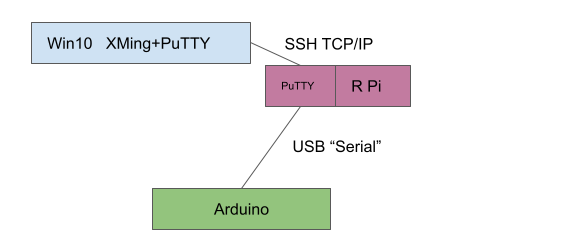
\includegraphics[width=.5\textwidth]{images/PuTTYDiagram1.png}
\caption[Win1X use.]{Win1X office desktop monitor uses TCP/IP and SSH
  with the -X switch to open a connection to Raspberry Pi. A PuTTY
  instance is started on the Raspberry Pi, configured for the USB port
  for the Arduino displays the PuTTY window on the remote desktop vi
  SSH -X working with Xming} %% \caption{{\tiny{citation}}}
\label{figure:Diagram1}
\end{figure}

\begingroup \fontsize{10pt}{10pt}
\selectfont
%%\begin{Verbatim} [commandchars=\\\{\}]
\begin{verbatim} 

Check the files in the /etc/X11 directory:
   /etc/X11/xinit/xserverrc
   ~/.xinitrc
   ~/.xsession  -- start programs when the login is complete
   ~/.profile

ssh-keygen -t ed25519 -C "your_email@example.com"

\end{verbatim}
\endgroup
%% \end{Verbatim}

If there is no /etc/X11


\verb=xmodmap -pke > ~/.Xmodmap # make a .Xmodmap upon which to hack=

This varies with new modern keyboards, there is massive
confusion over what a key is called and what code corresponds to
the key among keyboard vendors. 

To use the \dhl{caps lock} key as a spare \dhl{control} key find the
code for the caps lock key using the \dhl{xev} program. Xev will show
keycodes when a key changes state, like shift down, then shift up
etc...  

Hit the the ``caps'' key and note its code. Then edit the \dhl{~/.Xmodmap}
file and change:

\verb/keycode  37 = Control_L NoSymbol Control_L/



\newpage
\subsection{Remote Desktop PuTTY}

On the remote desktop, configure the remote PuTTY:

\vspace{-.15cm}
\begin{enumerate}\addtolength{\itemsep}{-0.5\baselineskip}
%\setcounter{enumi}{N}
   \item   Session:
\vspace{-.15cm}
\begin{enumerate}\addtolength{\itemsep}{-0.5\baselineskip}
%\setcounter{enumi}{N}
   \item   Select the \dhl{Serial} radio button
   \item   Serial Line to \dhl{/dev/ttyACM0}
   \item   Speed \dhl{9600}
   %\item   CTM\_X
   \item   Close window on exit $\rightarrow$ \dhl{Only on clean exit}
\end{enumerate}
   \item   Terminal
\vspace{-.15cm}
\begin{enumerate}\addtolength{\itemsep}{-0.5\baselineskip}
%\setcounter{enumi}{N}
   \item   In the \dhl{Line disipline options}:
\vspace{-.15cm}
\begin{enumerate}\addtolength{\itemsep}{-0.5\baselineskip}
%\setcounter{enumi}{N}
   \item  Local echo to \dhl{Force on}
   \item  Local line editing to \dhl{Force on}
\end{enumerate}
\end{enumerate}
   \item   Window
\vspace{-.15cm}
\begin{enumerate}\addtolength{\itemsep}{-0.5\baselineskip}
%\setcounter{enumi}{N}
   \item   Columns: \dhl{120} Rows: \dhl{50}
   \item   scrollback 200
   \item   display scrollbar
   %\item   Reset scrollback on display activity
   %\item   push erased text into scrollback
\end{enumerate}
   \item   Connection $\rightarrow$ Data
\vspace{-.15cm}
\begin{enumerate}\addtolength{\itemsep}{-0.5\baselineskip}
%\setcounter{enumi}{N}
   \item   login name can be set to \dhl{smate} for stellarmate, or
     the remote user's name.
   \item   Terminal-type string xterm
   \item   Terminal Speed 38400, 38400
\end{enumerate}
   \item   SSH$\rightarrow$X11
\vspace{-.15cm}
\begin{enumerate}\addtolength{\itemsep}{-0.5\baselineskip}
%\setcounter{enumi}{N}
   \item   Enable X11 forwarding
   \item   localhost:0.0
   \item   MIT-Magic-Cookie-1
\end{enumerate}
\vspace{-.15cm}
\begin{enumerate}\addtolength{\itemsep}{-0.5\baselineskip}
%\setcounter{enumi}{N}
   \item   Serial
\vspace{-.15cm}
\begin{enumerate}\addtolength{\itemsep}{-0.5\baselineskip}
%\setcounter{enumi}{N}
   \item   Baud to 9600
   \item   Data bits 8
   \item   Stop bits 1
   \item   Parity None
   \item   Flow Control None.
\end{enumerate}
\end{enumerate}

\end{enumerate}

\begin{figure}[h!]
\centering
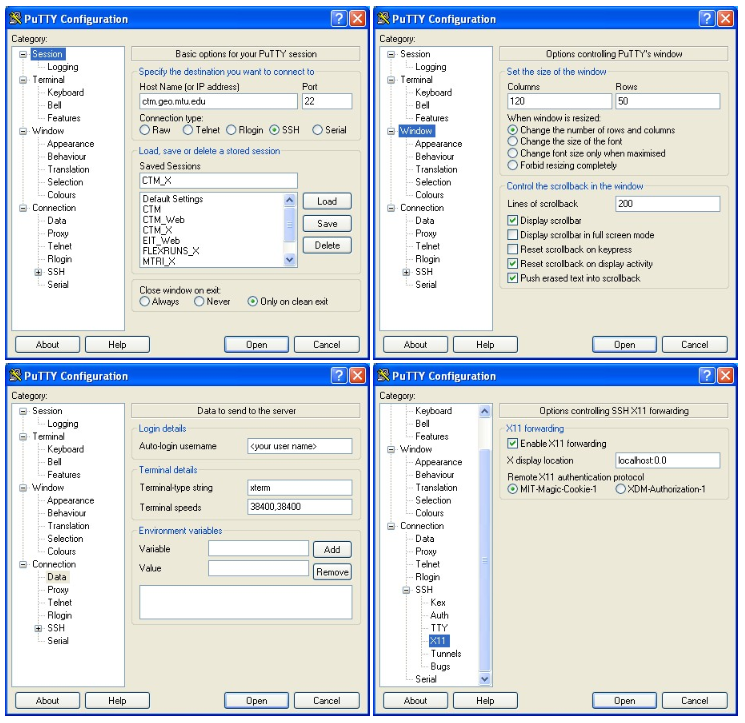
\includegraphics[width=.7\textwidth]{images/PuYYTXming.png}
\caption{PuTTY screen snaps of the 4 configuration menu panels.} %% \caption{{\tiny{citation}}} 
\label{figure:}
\end{figure}



\newpage
\subsection{Remote Desktop Xming}


On the Windows pane, enter a new configuration for this machine.

\vspace{-.15cm}
\begin{enumerate}\addtolength{\itemsep}{-0.5\baselineskip}
%\setcounter{enumi}{N}
   \item Page 1 - Set Multiple windows (Each remote application gets
     its own Win1X office desktop window).
   \item Page 2 - Start no client. The clients are started with the
     Win1X PuTTY's SSH -X session.
   \item  Page 3 - Clipboard (handy)
   \item Page 4 - Save the configuration. This sets the policy for all
     machines, Xming does not care about the remote machines business
     -- any remote may connect if firewall permissions are set.
\end{enumerate}


\begin{figure}[h!]
\centering
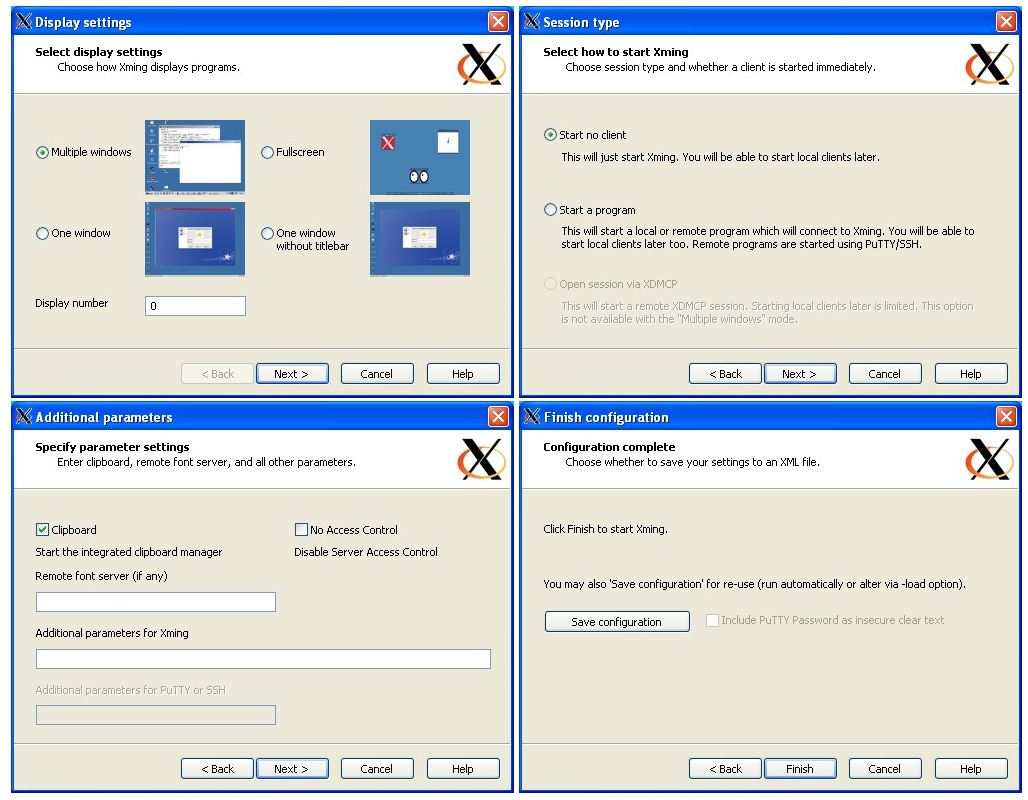
\includegraphics[width=.75\textwidth]{images/XmingConfig.png}
\caption{Xming screen snaps of the 4 configuration menu panels.} %% \caption{{\tiny{citation}}} 
\label{figure:}
\end{figure}


\newpage
\section{SSH on the Raspberry Pi}

Note: this section is complicated by the details needed to open
home firewalls to the internet using the local Telco's interface
routers. Each router is different, and the Telco changes its mind
frequently.

This command will list the full name for hosts that are on the network.
Here we're looking for our machine \dhl{pier15} that will appear
as \dhl{pier15.hsd1.co.comcast.net}:

{\color{verbcolor}{\verb={sudo nmap -sP 10.1.10.0/24 | awk -e '/\^Nmap/ {print $5;}'}=}}

If ssh issues a 

\dhl{ssh: connect to host <machine>.local port 22: Connection refused}

use the keyboard/mouse for the raspbian machine and run the command
\dhl{sudo raspi-config}, then under Interface options, \dhl{I2 SSH} tab, enable.


SSH (Secure SHell), originates on port 22. The port needs to be allowed
through the Raspbian's ``uncomplicated firewall'' \dhl{ufw} task. Root
permissions are required.

\begingroup \fontsize{10pt}{10pt}
\selectfont
%%\begin{Verbatim} [commandchars=\\\{\}]
\begin{verbatim} 
sudo ufw list       # see all the current ports
sudo ufw allow ssh  # allow the port to work.
\end{verbatim}
\endgroup
%% \end{Verbatim}

\subsection{Raspberry Pi -- Raspbian SSH}

Enable SSH through the Raspberry Pi Configuration menu:
\dhl{Preferences $\rightarrow$ Raspberry Pi Configuration} Click on ``Interfaces'':
and select \dhl{Enabled} next to SSH.

Use the command \dhl{sudo nano /etc/ssh/sshd\_config} find
and X11Forwarding set the value to yes \dhl{ X11Forwarding yes}.

Save.

\dhl{sudo systemctl restart ssh}

% https://techsphinx.com/raspberry-Pi/enable-x11-forwarding-on-raspberry-Pi/

\subsection{StellarMate}

You need to \dhl{sudo apt update}, then \dhl{sudo apt install putty -y}
to install PuTTY.

The ssh connect to StellarMate is made to an alternate port:

\dhl{ssh -X -p 5624 stellarmate@stellarmate.local}

The username is stellarmate and the password is the usual stellarmate password.

\section{Using Putty from Linux Desktop} \label{sec:LinuxDesktop}

PuTTY on a linux desktop machine in the office has all the Xming features
built-in and does not require additional X-windows code.

\section{Linux Ports}

Linux treats devices like serial ports, USB ports etc as special
files. Making no distinction makes things very easy but drives
Win1X people nuts.

The ports you are interested in:

\vspace{-.15cm}
\begin{enumerate}\addtolength{\itemsep}{-0.5\baselineskip}
%\setcounter{enumi}{N}
   \item   /dev/serial0 - the serial port pins on the Raspberry Pi. This requires 
special action to enable the GPIO pins. This is recognized by the Arduino on its Serial1
 device.
   \item   /dev/ttyAMC0 - the USB port recognized by the Arduino on its Serial
 device.
\end{enumerate}

\section{Running the Arduino CLI on the Raspberry Pi}

The Raspberry Pi will run the Arduino CLI, which in turn may run a
serial port connection. Using the magic of X11, discussed above, the
Arduino CLI windows will appear on the Win1X office desktop monitor or
Linux office desktop monitor.

From the Win1X machine:

\vspace{-.15cm}
\begin{enumerate}\addtolength{\itemsep}{-0.5\baselineskip}
%\setcounter{enumi}{N}
   \item   Use Xlaunch with multiple windows.
   \item   Then make a PuTTY connection to the RPi. (Call this Win1X/Rpi)
\vspace{-.15cm}
\begin{enumerate}\addtolength{\itemsep}{-0.5\baselineskip}
%\setcounter{enumi}{N}
   \item   this opens a Win1X cmd window, and prompts for the password into
 the RPi machine.
   \item   A Rpi prompt will appear.
\end{enumerate}

   \item   In the Win1X/Rpi window (now a shell on the RPi)
\vspace{-.15cm}
\begin{enumerate}\addtolength{\itemsep}{-0.5\baselineskip}
%\setcounter{enumi}{N}
   \item   enter the command \dhl{putty {-}{-}display=\$DISPLAY} (two dashes)
   \item   This causes a PuTTY configuration window from the RPi to appear on the 
           Win1X desktop.
   \item   Configure for the serial connection desired \dhl{/dev/ttyAM0} for
          the Arduino.
\end{enumerate}

\vspace{-.15cm}
\begin{enumerate}\addtolength{\itemsep}{-0.5\baselineskip}
%\setcounter{enumi}{N}
   \item   Run
   \item   This causes a PuTTY serial console (as you configured it) to appear on the
 Win1X desktop.
   \item   Interact with the Arduino, at the end of a UART serial connection, with
   the FlexSpec1 instrument -- as though you were at the Rpi.
\end{enumerate}
\end{enumerate}


You may wish to install \dhl{xeyes} program on the RPi. Xeyes 
is a rather simplistic X11 program that causes a little window
to pop-up with two ``eyeballs'' where the ``eyes'' will watch the
mouse move around. This tests mouse and graphics in on go. To
do so -- in the Win1X/Rpi console enter: 

\begingroup \fontsize{10pt}{10pt}
\selectfont
%%\begin{Verbatim} [commandchars=\\\{\}]
{\color{verbcolor}
\begin{verbatim} 
sudo apt install x11-utils
\end{verbatim}
}
\endgroup
%% \end{Verbatim}


\subsection{Additional Resources}

\url{http://www.straightrunning.com/xmingnotes/IDH_PROGRAM.htm}

\subsection{More than One Win1X connection}

Make Desktop Icon's for unique connections:


\vspace{-.15cm}
\begin{enumerate}\addtolength{\itemsep}{-0.5\baselineskip}
%\setcounter{enumi}{N}
   \item  Run XLaunch.exe and save the configuration to file config.xlaunch.
   \item  Create a shortcut of XLaunch.exe under Startup directory.
   \item Modify the target field of the shortcut to
     \verb="C:\ZZH\software\Xming\XLaunch.exe" -run "config.xlaunch"=.
\end{enumerate}

\subsubsection{Another approach to autostart with Win1X}
\vspace{-.15cm}
\begin{enumerate}\addtolength{\itemsep}{-0.5\baselineskip}
%\setcounter{enumi}{N}
   \item  Search for Xming in the Start Menu
   \item  Right click on the shortcut and select Open file location
   \item  Copy the selected Xming shortcut
   \item  Press Ctrl-l to move the cursor to the Explorer location input
   \item  type shell:startup and then Enter
   \item  Paste the Xming shortcut in the Startup directory.
\end{enumerate}

\section{Auditing}

It is possible to save the and/or share the configuration parameters
for PuTTY.

\subsection{Windows}

PuTTY on Win1X records its configuration(s) into the Registry. It
requires the dangerous step of using Regedit to recover. The steps are:

\vspace{-.15cm}
\begin{enumerate}\addtolength{\itemsep}{-0.5\baselineskip}
%\setcounter{enumi}{N}
   \item   Find  \verb=HKEY_CURRENT_USER\Software\SimonTatham\PuTTY=
  Note: The ``SimonTatham'' is the name of the author of the package
  not you, the ``CURRENT\_USER''.
   \item   Right click and export, the resulting file is a text file suitable
  for sharing and archiving.
\end{enumerate}


\subsection{Linux}

The configuration file is in \dhl{\$HOME/.putty} deep.






% hostname to stellarmate  port 5624


%% use a bibitem approach to the references publications etc.
%% (wg-bibitem)

%%\clearpage
\addcontentsline{toc}{section}{References}
\renewcommand*{\refname}{My Bibliography and References}
\bibliographystyle{apalike}	% bibliographystyle{apalike} and \usepackage{natbib}
\bibliography{MasterBib}	% expects file "MasterBib.bib"



%%\begin{thebibliography}{80}
%%\usepackage{natbib}   %% bibitems
%%\end{thebibliography}

%%\clearpage
\addcontentsline{toc}{section}{Index}
\printindex %% www.cs.usask.ca/resources/tutorials/latex/notes/toc-index.pdf

%% (wg-texdoc-endnotes)

%%%%%%%%%%%%%%%%%%%%%%%%%%%%%%%%%%%%%%%%%%%%%%%%%%%%%%%%%%%%%%%%%%%%%%%%%%%%%
% Support for endnotes
%% \begingroup
%% \renewcommand{\notesname}{\textcolor{red} {Action Items:}}
%% \parindent 0pt
%% \parskip 2ex
%% \phantomsection
%% \addcontentsline{toc}{section}{	extcolor{red} {Action Items:}}
%% \def\enotesize{\normalsize}
%% \theendnotes
%% \endgroup

\end{document}
